%!TEX root = ../report.tex
\chapter{System Context}
\label{ch:context}

In this chapter the context of Docker is presented.

\subsection{System Context}
Docker is a open-source-software designed with the purpose of making the deployment of distributed application easier.
 " Docker provides an integrated technology suite that enables development and IT operations teams to build, ship, and run distributed applications anywhere."
It " automates the deployment of applications inside software containers, by providing an additional layer of abstraction and automation of operating-system-level virtualization on Linux ". \\
The first open-source version was released in March 2013. \\
It's written in the Go Programming language. \\

Sources : \textit{https://www.docker.com/what-docker}
%\textit{https://en.wikipedia.org/wiki/Docker_\%28software\%29#History}

\begin{figure}[H]
\centering
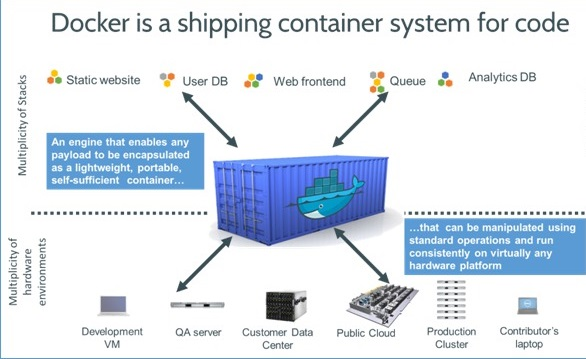
\includegraphics[scale=0.8]{images/docker_container.jpeg}
\caption{Docker}
\label{fig:analysis-mvc}
\end{figure}

\subsection{Community}
Docker started as an internal project within dotCloud, a platform-as-a-service company with four main developpers. \\
The following organizations are the main contributors to Docker: the Docker team, Red Hat, IBM, Google, Cisco Systems and Amadeus IT Group. \\